%==============================================================================
\chapter{The Large Hadron Collider and the ATLAS Experiment}
\label{sec:ATLAS}
%==============================================================================

\section{The Large Hadron Collider}
\label{sec:LHC}
The Large Hadron Collider (LHC) is the world's largest particle accelerator. It's located at the European nuclear research center CERN at the french swiss border near Geneva. The construction of the collider started in 2000, along the $\SI{27}{km}$ long tunnel of its predecessor, the Large Electron-Positron Collider (LEP). Over ten thousand scientists from more than 100 countries contributed to its construction. The LHC was designed to collide protons with a center of mass energy of $\sqrt{s}= \SI{14}{TeV}$, to push the limits of our understanding of particle physics, conditions similar to those of the very early universe. \\
During Run 1 of the LHC in the years 2010 to 2012 a center of mass energy of $\sqrt{s}= 7-\SI{8}{TeV}$ was reached. The most famous discovery made during this time period is the observation of the last missing ingredient of the SM, the Higgs boson in 2012 by the ATLAS and CMS collaborations \cite{Higgs}. After two years of construction work, Run 2 started in 2015 and ended in 2018. During Run 2, properties of the Higgs boson such as its Yukawa coupling to the heaviest, third-generation quarks and leptons were investigated. Moreover, many precision measurements of SM parameters were executed to search for physics beyond the Standard Model (BSM). \\


\begin{figure}[H]
\centering
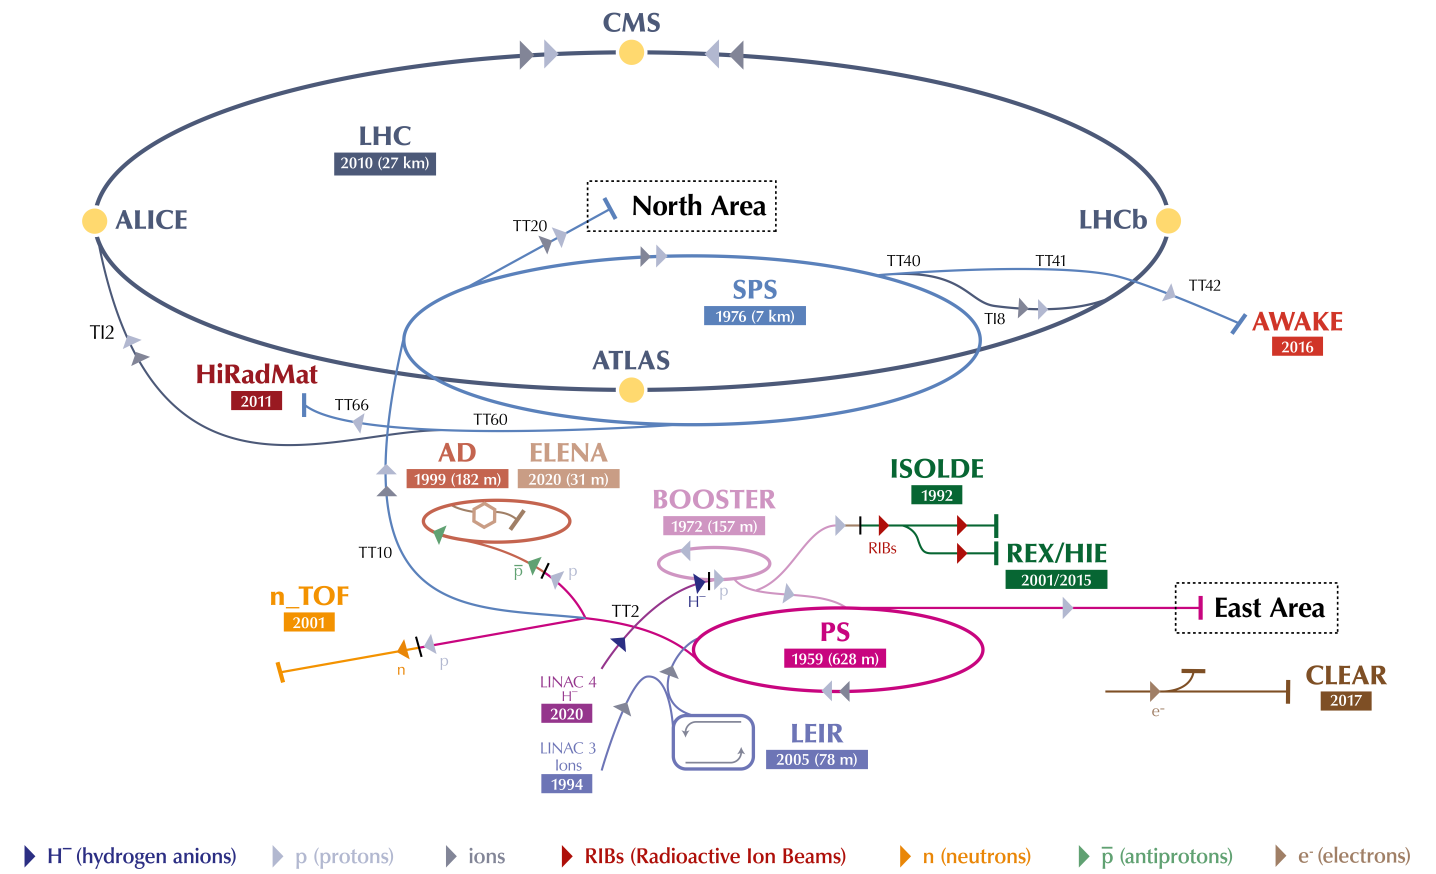
\includegraphics[scale=0.215]{Cern}
\caption{The accelerator complex of CERN including the LHC. The accelerator chain for the protons is shown as well as the four major experiments.\cite{CernAcc}}
\label{fig:Cern}
\end{figure}

\newpage

\paragraph{Proton Acceleration} \mbox{} \\

The protons that will be accelerated to the TeV energies originate from hydrogen atoms in a bottle. After their ionization, the protons are pre-accelerated to $\SI{450}{GeV}$, and squeezed into \textit{bunches}. The three pre-accelerators Linac 2, PSB, and SPS are shown in Figure \ref{fig:Cern}. The bunch trains of protons entering the LHC are separated by \SI{25}{ns} and containing $1.15\cdot 10^{11}$ protons. They are further accelerated by electrical fields and focused via magnetic fields of $\SI{3}{T}$ provided by superconducting dipole and quadrupole magnets. The LHC itself consists of two parallel vacuum rings in which protons travel in opposite directions. Once the protons have reached the desirable energy, they collide at 4 interaction points. At each point, one detector is located, namely ATLAS, CMS, ALICE, and LHCb. The ATLAS and CMS detectors are general-purpose detectors looking for particle properties and BSM physics. The LHCb experiment is the only fixed target experiment at CERN and is focused on heavy flavour physics. The fourth experiment ALICE studies heavy-ion physics such as quark-gluon plasma. \\

\paragraph{Luminosity and Pile-up} \mbox{} \\

Rare high energetic processes such as $t\bar{t}t\bar{t}$ can only be observed if the center of mass energy is high and enough particle collisions take place. If a collider produces the required number of events is quantified by its Luminosity $L$. It's defined by the formula
\begin{equation}
\label{eq:Lumi}
L = \frac{1}{\sigma} \frac{dN}{dt} \cdot \epsilon \,  \,; \, \,\,\,\,\,\,\,\,\, [L] = \text{m}^{-2}\text{s}^{-1}=\text{fb}^{-1}
\end{equation}
where $\sigma$ is the cross-section, giving the number of events that are recorded per unit area and $\epsilon$ the detector efficiency defined as the fraction of events which are measured in the detector relative to the number of events produced. The design Luminosity of the LHC is $L = \SI[parse-numbers=false]{10^{34}}{m}^{-2}\text{s}^{-1}$, however, it has been surpassed during Run 2. Of practical importance is the integrated Luminosity $\mathcal{L}$
\begin{equation}
\mathcal{L} = \int L dt
\end{equation}
since the Luminosity add up with time and can vary depending on collider conditions. One drawback of high Luminosities is that multiple interactions at the same bunch crossing take place. However, only the interaction with the highest energy is of interested called the \textit{hard scattering event}. All events originating from other interactions are called \textit{pile-up} $<\mu>$. In practise its a challenging task to identify and remove particles coming from pile-up.

\section{The ATLAS Experiment} 
\label{ATLAS}
The ATLAS detector is the largest general-purpose detector at the Large Hadron Collider. Its main purpose is to search for new undiscovered particles and probe the SM by taking advantage of the high energetic protons available at the LHC. This section introduces the coordinate system and the structure of the ATLAS experiment as well as the particle reconstruction. \\


\paragraph{The ATLAS Coordinate System} \mbox{} \\
The coordinate system of the ATLAS experiment is right-handed with its origin at the interaction point. The z-axis is orientated in the direction of the beam pipe while the x-axis points to the center of the LHC, the points upwards. Cylindrical coordinates (z,$\Phi$,$\theta$) are a natural choice where $\Phi$ is the azimuthal angle around the beam pipe and $\theta$ the polar angle. A commonly used variation of $\theta$ is the pseudorapidity $\eta$
\begin{equation}
\label{eq:eta}
\eta = - \ln[\tan(\frac{\theta}{2})]
\end{equation}
where $\eta =0$ corresponds to the center of the detector and $\eta \rightarrow 0$ points to the beam axis. The advantage of this definition is that the outgoing particle rate per unit $\eta$ is on average constant. \\
The proton-proton collisions at the interaction point break up the inner structure of the protons resulting in new particles and particle \textit{jets}.\textit{Jets} in the context of particle physics refers to narrow cones of hadrons and other particles produced during the hadronization of quarks or gluons. The particles originating from the proton-proton have to have a total transverse momentum $p_{\text{T}}=p_{\text{x}}+p_{\text{y}}$ of zero since the partons of the initial protons, quarks and gluons, have negligible momenta in the transverse plane due to their high boost in the z-direction.

\paragraph{Inner Detector} \mbox{} \\

\begin{figure}[H]
\centering
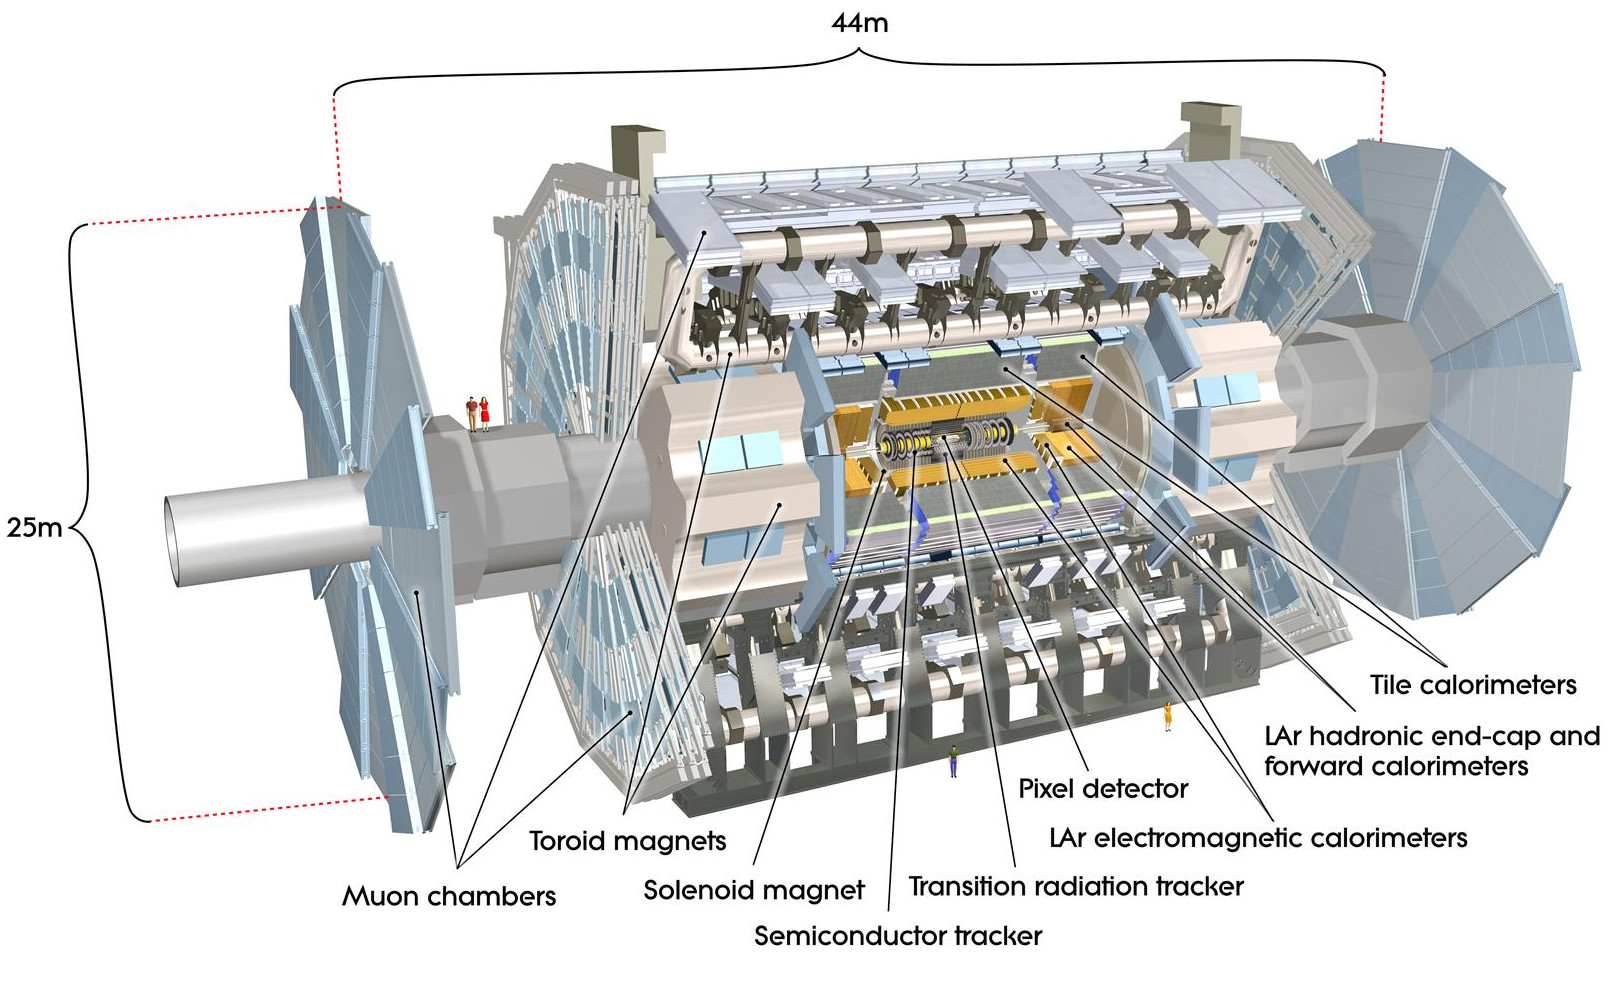
\includegraphics[scale=0.2]{ATLAS}
\caption{Illustration of the ATLAS detector and its sub-units.\cite{ATLASP}}
\label{fig:ATLAS}
\end{figure}

The track, momentum, and energy of particles are measured in cylindrically arranged detector layers surrounding the beam pipe, as shown in Figure \ref{fig:ATLAS}. The layer closest to the interaction point is called the inner detector and covers a pseudorapidity range of $|\eta| < 2.5$. It's composed of several highly granulated tracking detectors such as silicon pixel detectors and transition radiation detectors for particle identification. The super-conducting solenoid magnets provide a $\SI{2}{T}$ magnetic field in which the trajectory of charged particles are bent. The radius of this curve together with the tracking information provided by the inner detector can then be used to measure the particles momenta. 

\paragraph{Calorimeters} \mbox{} \\
The calorimeter of the ATLAS experiment enables the measurement of particle energies through interactions with the detector material. Particles entering the calorimeters initiate showers until they are stopped. The length of these showers is proportional to the energy deposited by the particle. The ATLAS calorimeter system consists of two different calorimeters an electromagnetic calorimeter (ECAL) and a hadronic calorimeter (HCAL). Showers initiated in the ECAL are governed by the electroweak interaction, therefore, the chosen material is a gas (liquid  Argon). On the other hand, the HCAL contains scintillator crystals adjusted for the hadronic showering. The pseudorapidities covered by the ECAL are $1.36 < |\eta| < 3.2$ and $1.7 < |\eta| < 3.2$ for the HCAL, excluding the \textit{crack region} $1.3 < |\eta| < 1.52$ between the barrel and the end cap.

\paragraph{Muon Spectrometer} \mbox{} \\
The outermost layer of the ATLAS detector is the muon spectrometer. Muons are Minimum Ionizing Particles (MIPs) for a range for $\mathcal{O}(100)$ MeV up to the TeV scale. Therefore, they only deposit a small fraction of their energy in the calorimeters. To identify and measure the properties of muons, gaseous detectors in a magnetic field are used. A muon passing through such a detector ionizes the gas. The ions and electrons drift in an electrical field and induce a signal. The muon spectrometer of the LHC has a magnetic field of $\SI{0.5}{T}$ to $\SI{1}{T}$ and covers a range of $|\eta| < 2.7$.


\paragraph{Object reconstruction} \mbox{} \\

\begin{figure}[H]
\centering
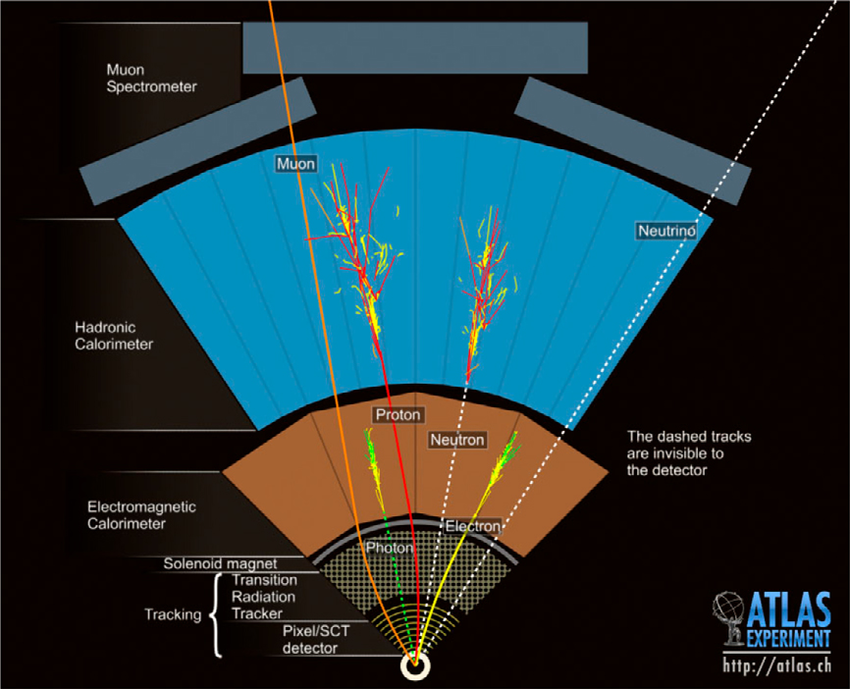
\includegraphics[scale=0.8]{ATLAS_interactions}
\caption{Interaction of different types of particles with different segments of the ATLAS detector.\cite{ATLASint}}
\label{fig:Interaction}
\end{figure}

The detector signals of the different particles (cf. Figure \ref{fig:Interaction}) have to be converted into physics objects. Since many particles such as the top quark or W and Z bosons decay before reaching the detector they have to be identified via their long-living decay products. A process referred to as reconstruction. Notably, the reconstruction of most physics objects is performed independently. The overlap removal is then performed dependent on the goal of the analysis carried out. \\
While leptons, photons, and jets can be identified by their interaction with the different detector components, neutrinos do not interact with any part of the detector. They have to be identified via the conservation of transverse momentum. The deviation of the total $p_{\text{T}}$ sum from zero is an indication for the presence of neutrinos or other exclusively weakly interacting BSM particles. The missing transverse momentum can be defined as
\begin{equation}
\label{eq:Etmis} 
E_{\text{T}}^{\text{miss}} = - \sum_{i \in {\text{final state particles}}} p_{\text{T},i}
\end{equation}
Of special interest for the reconstruction of top quarks, and thus the $t\bar{t}t\bar{t}$ process, are the b-jets originating from the hadronization of b quarks. The B hadrons contained in the b-jets have a long lifetime and usually decay within the tracking detectors. Therefore, a secondary decay vertex can be identified. To improve the efficiency of b-tagging further, kinematic properties such as the mass and the fragmentation of B Hadrons are utilized. 
